\documentclass{article}
\usepackage[utf8]{inputenc}
\usepackage{graphicx}
\usepackage{float}
\usepackage{courier}

\title{Visualization of the Knee}
\author{Christian aan de Wiel (10737499)}
\date{\today}

\begin{document}

\maketitle

\begin{abstract}
In this report, an interactive piece of software is explained and shown. A knee from a healthy female is visualized in multiple ways, namely volumetric rendering, volumetric slicing and mesh rendering. Segmentation is performed using an evolutionary region growing algorithm implemented in ITK.
\end{abstract}

\section{Introduction}
This report describes an approach to visualizing a 3T MRI scan of a healthy female knee with an emphasis on anatomical segmentation. The dataset contains voxel data with dimensions 256x256x32 and consists of 7 different scans. The application should have a user interface, two different visualization methods and be able to distinguish different anatomical structures in the knee.

\section{Method}
This section will describe the implemented visualizations options and features of the source.

\subsection{General overview}
The application has two different renderers, a 3D and a 2D renderer. The 3D renderer visualizes the segmentation, while the 2D renderer allows for a more accurate way of measuring tissues. The pipeline of the 3D renderer contains two main rendering methods, namely volumetric raycasting and regular mesh rendering. The 2D window uses an adapted version of volumetric rendering, where only one slice is constructed and displayed in two dimensions.
\begin{figure}[H]
    \centering
    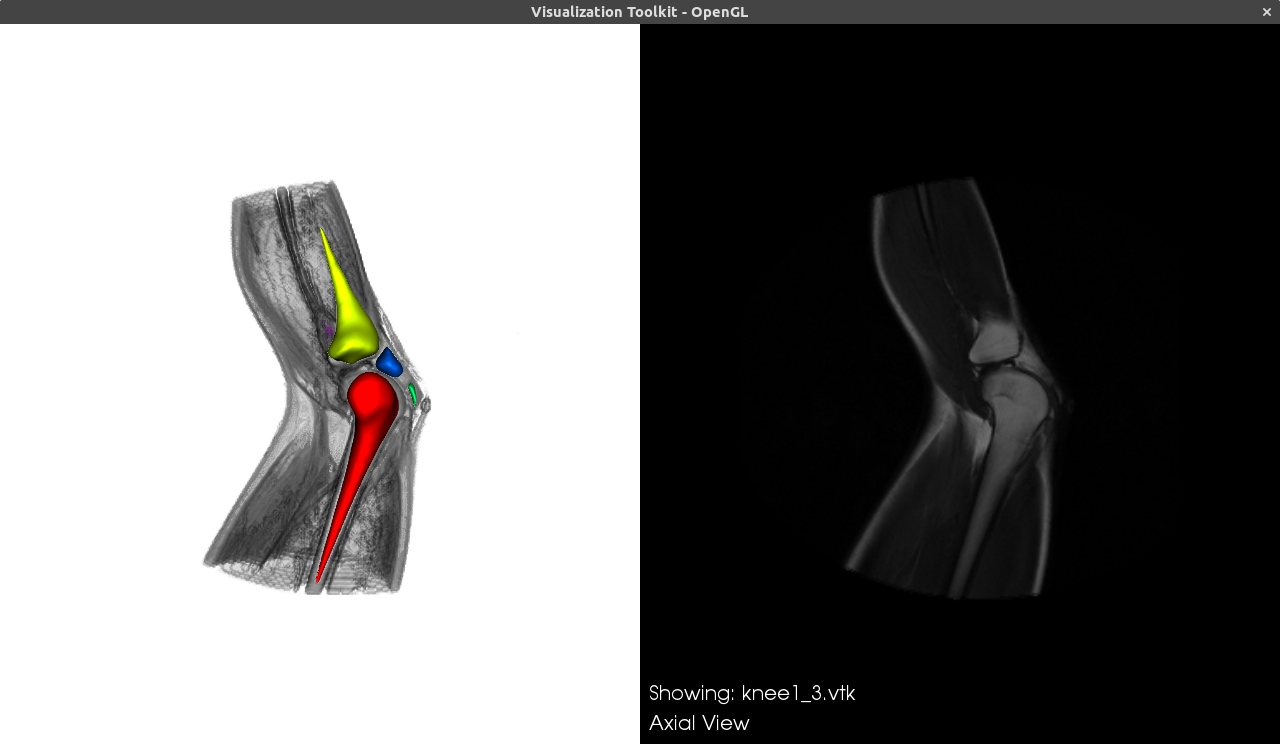
\includegraphics[width=\textwidth]{graphics/general.png}
    \caption{General overview of the application.}
    \label{fig:my_label}
\end{figure}

\subsection{Segmentation}
Segmentation is performed as pre-processing step on the dataset using ITK, ITK-SNAP\footnote{http://www.itksnap.org/pmwiki/pmwiki.php} to be precise. The segmentation process consists of a few different steps. First of all, the region of interest (ROI) is defined. This is a 3D bounding box that allows/restricts certain parts of the volumetric data to be taken into account.

The second step is pre-segmentation. In this step, the data is segmented using a high level method (e.g. thresholding, classification, clustering and edge attraction). For this dataset, thresholding seemed to perform best. A visualization of this process, can be seen in figure \ref{fig:presegmentation}.
\begin{figure}[H]
    \centering
    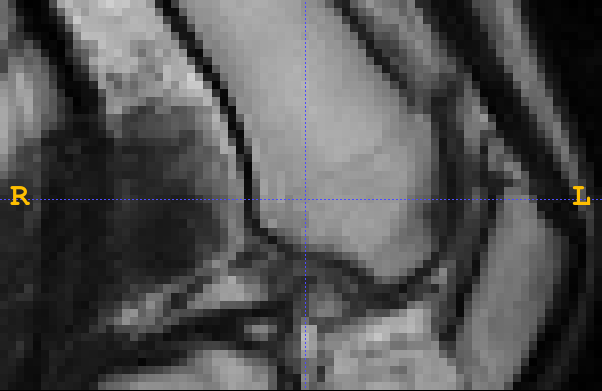
\includegraphics[width=0.49\textwidth]{graphics/pre_segmentation_1.png}
    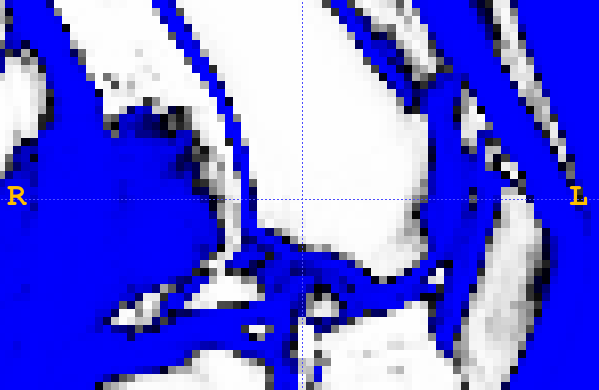
\includegraphics[width=0.49\textwidth]{graphics/presegmentation_2.png}
    \caption{Pre-segmentation: Volumetric data before thresholding (left) and after thresholding (right).}
    \label{fig:presegmentation}
\end{figure}

The third step is called initialization. Here, we place region growing seeds/bubbles to hint the segmentation algorithm which part of the data we actually want to be segmented (we do not want all the white regions in figure \ref{fig:presegmentation}). This process is visualized in figure \ref{fig:initialization}.
\begin{figure}[H]
    \centering
    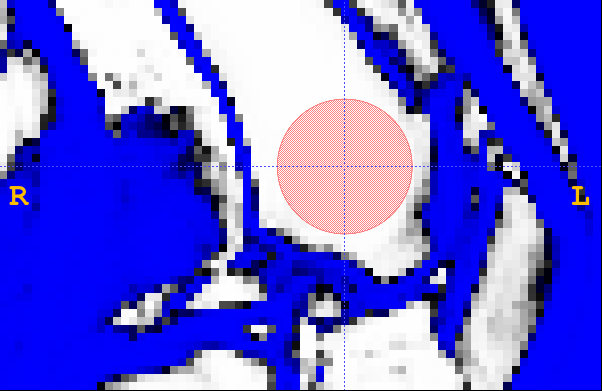
\includegraphics[width=0.5\textwidth]{graphics/initialization.png}
    \caption{Initialization: In red a region growing seed/bubble is shown.}
    \label{fig:initialization}
\end{figure}

The last step is evolution. Here the bubble grows in all three dimensions and is restricted by the result of the pre-segmentation (the bubble will not evolve in the blue color, only the white color).
\begin{figure}[H]
    \centering
    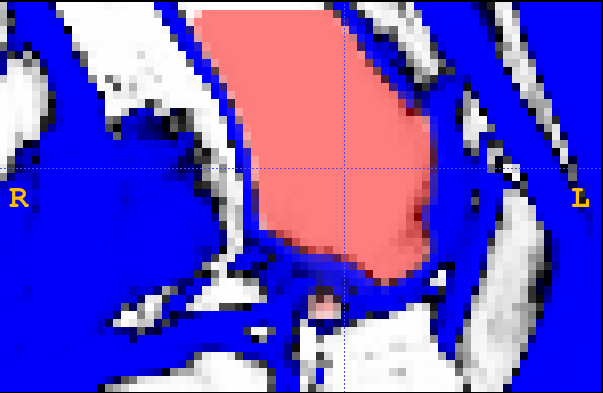
\includegraphics[width=0.55\textwidth]{graphics/evolution_1.png}
    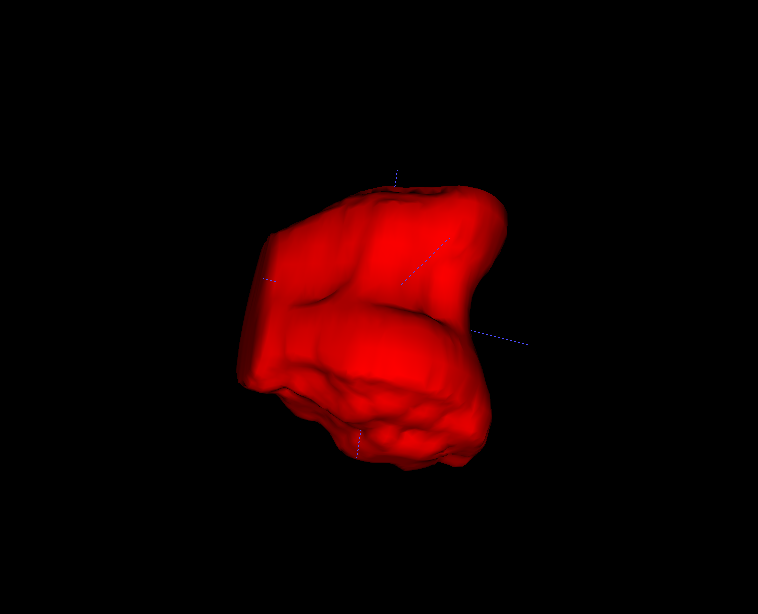
\includegraphics[width=0.44\textwidth]{graphics/evolution_2.png}
    \caption{Evolution: Segmentation result in 2D (left) and 3D (right).}
    \label{fig:evolution}
\end{figure}

\subsection{Mesh Rendering}
Afterwards, these segmentation can be exported as mesh in both VTK and STL format. The \texttt{vtkSTLReader} and \texttt{vtkPolyDataReader} can both read these segmentations. To make the segmentations more appealing and aesthetic, the mesh rendering pipeline contains several different filters.

First of all, ITK-SNAP exports the mesh in a flipped world space, so a \texttt{vtkTransformPolyDataFilter} should be used to flip it back. Afterwards a \texttt{vtkSmoothPolyDataFilter} is used to smooth the data. Finally, specular rendering is enabled and interpolation is set to phong (this requires computing the normals of the polydata with \texttt{vtkPolyDataNormals}). Each segmentation is rendered in a different color. The result can be seen in figure \ref{fig:only_segmentations}.

\begin{figure}[H]
    \centering
    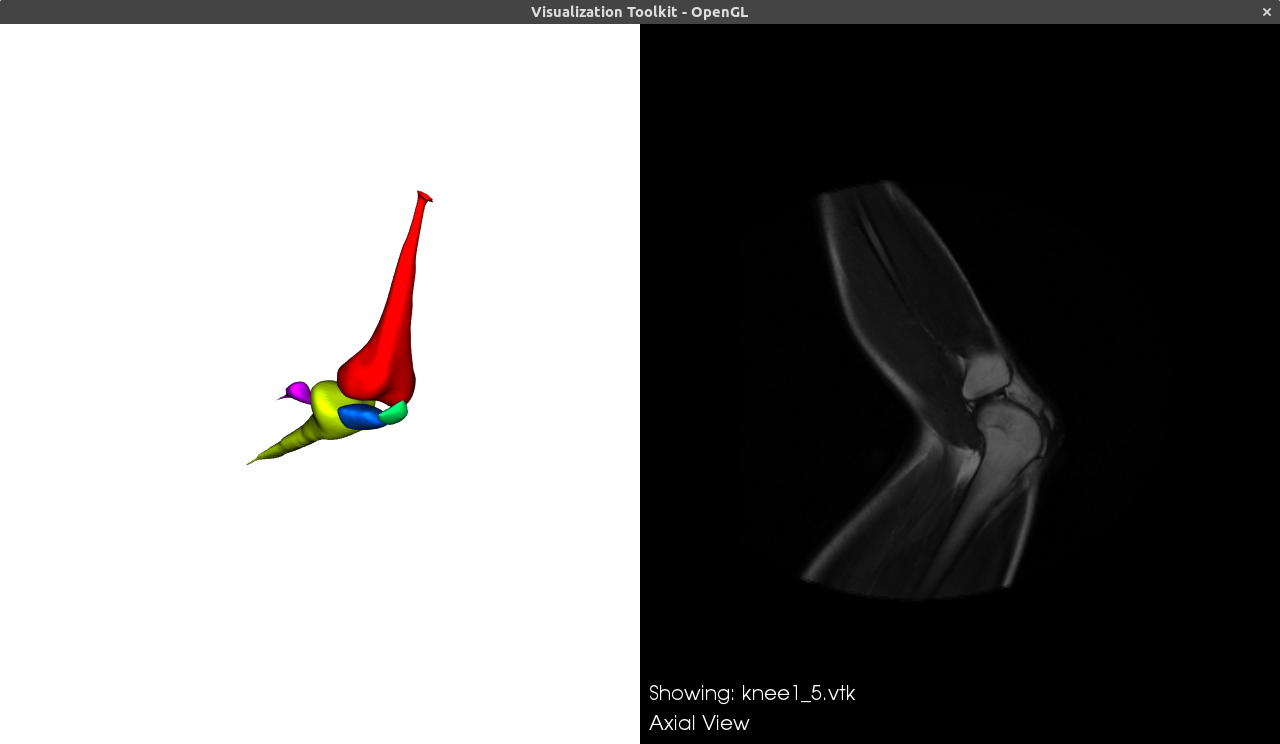
\includegraphics[width=\textwidth]{graphics/only_volume.png}
    \caption{Caption}
    \label{fig:only_segmentations}
\end{figure}

\subsection{Volumetric Rendering}
In order to see all different tissues, volumetric rendering is used. The predefined transfer function sets the opacity of the segmented tissues to 0.9 (the value range has been derived using VolView). This ensures that the mesh segmentation are well defined and easy to spot. Afterwards, \texttt{vtkOpenGLGPUVolumeRayCastMapper} is used to map the volume to the actor.

In order to create an axial, coronal, saggital and oblique view of the data, \texttt{vtkImageReslice is used} (this method is based on one of the VTK examples\footnote{https://github.com/Kitware/VTK/blob/master/Examples/ImageProcessing/Python/ImageSlicing.py}). The slice orientation is one of the 4D matrices that corresponds with the right slice orientation. The colors are mapped to the volumetric data using a lookup table. The result of these 2D slices of the volumetric data can be seen in \ref{fig:slicing}.

\begin{figure}[H]
    \centering
    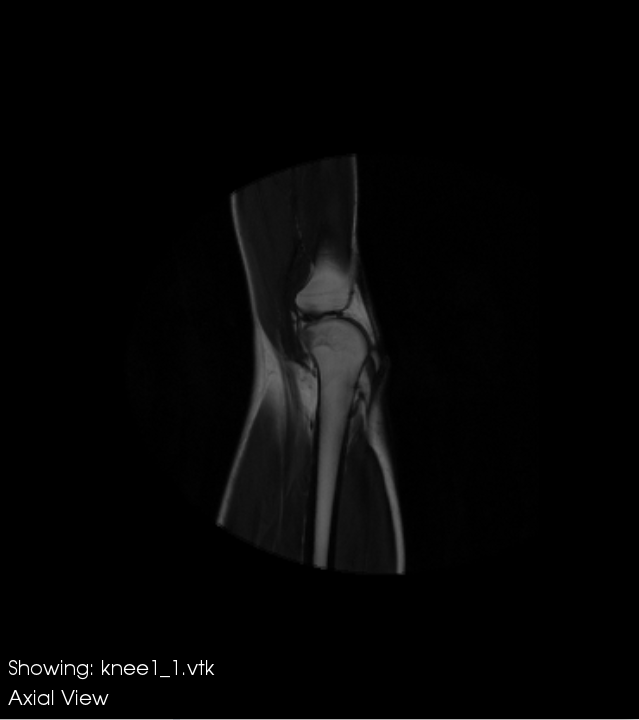
\includegraphics[width=0.49\textwidth]{graphics/axial.png}
    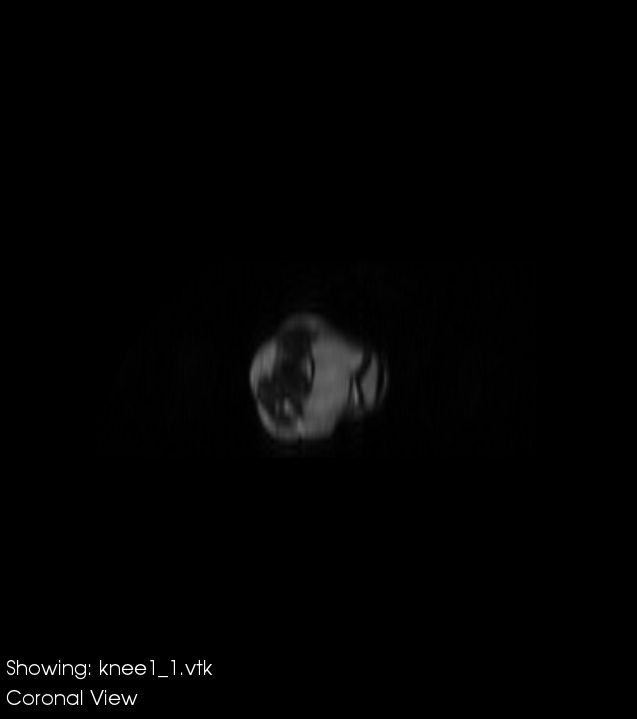
\includegraphics[width=0.49\textwidth]{graphics/coronal.png}
    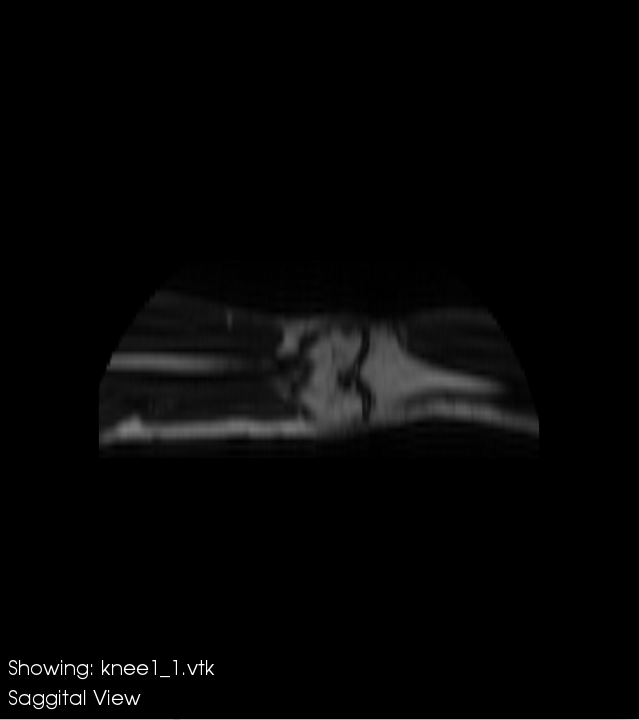
\includegraphics[width=0.49\textwidth]{graphics/saggital.png}
    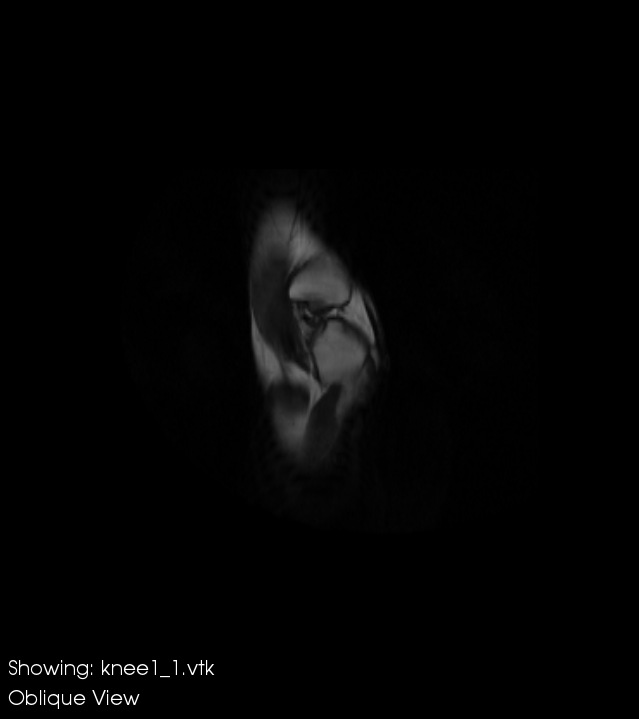
\includegraphics[width=0.49\textwidth]{graphics/oblique.png}
    \caption{From left to right, top to bottom: Axial, coronal, saggital and oblique view.}
    \label{fig:slicing}
\end{figure}

\subsection{Measuring}
Measuring has been implemented using raycasting. When the user presses the (VTK pre-defined) pick key, a ray is shot towards the users' mouse and a point is placed at the intersaction with the data. This can be done both in 3D and 2D, however, I found it easier and more precise to use the 2D representation for measuring. The user can pick two points and afterwards the Euclidian distance is calculated between the points. The result of measuring the femur bone can be seen in figure \ref{fig:distance}.
\begin{figure}[H]
    \centering
    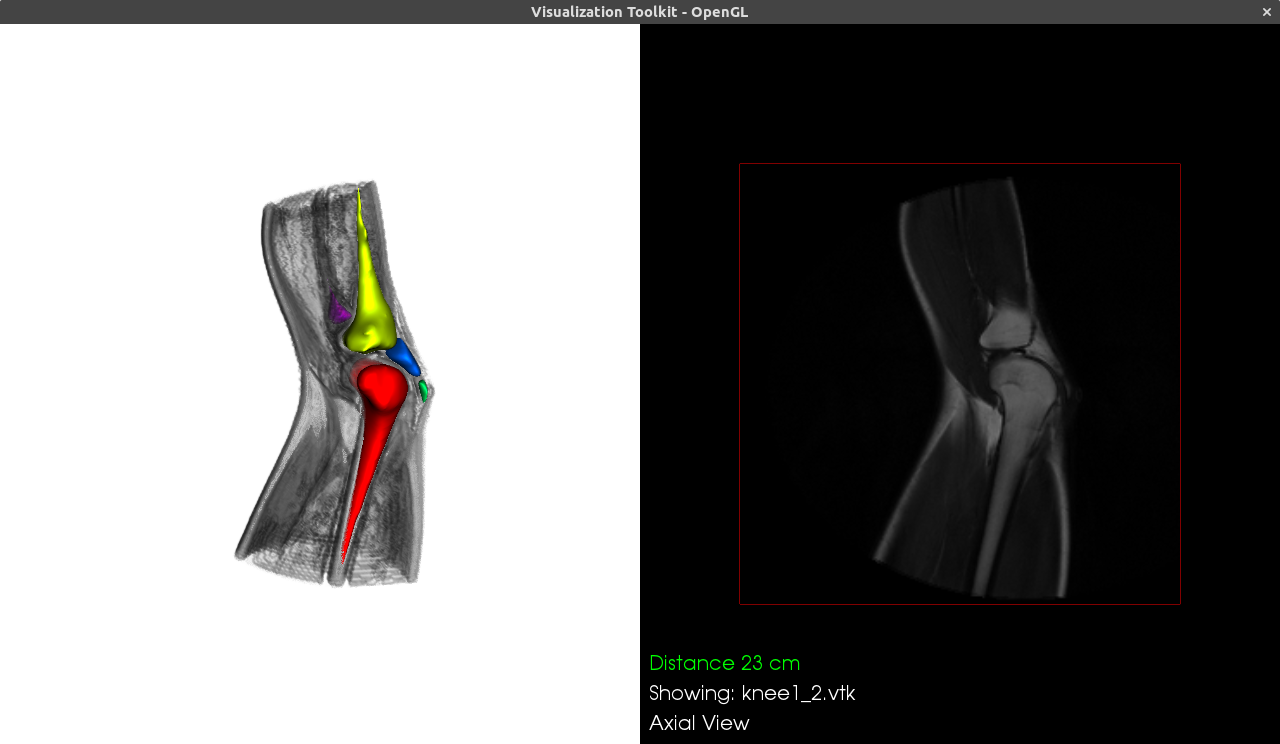
\includegraphics[width=\textwidth]{graphics/distance.png}
    \caption{Measuring the distance of the femur bone.}
    \label{fig:distance}
\end{figure}

\subsection{UI/Controls}
\begin{figure}[H]
    \centering
    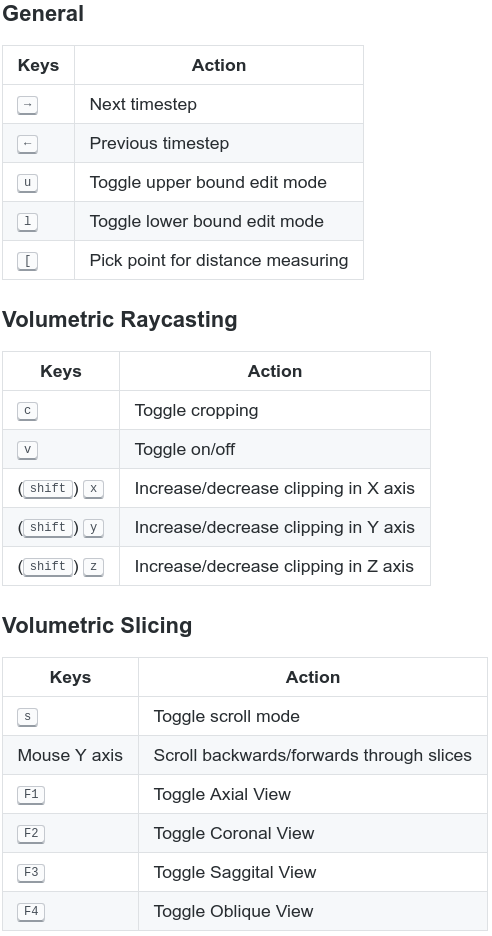
\includegraphics[width=0.7\textwidth]{graphics/controls.png}
\end{figure}

\section{Discussion and Conclusion}
This report describes an application that effectively visualizes a dataset of a human knee. The segmentation algorithm used to pre-process the data has shown to be effective and extremely powerful for segmenting these kinds of data. It would have been better to implement the segmentation using ITK and predefine the region growing seeds, however, this proved to be rather difficult (I got the VTK + ITK pipeline to work, however, the segmentation results were extremely poor) and as described by the assignment, beyond the scope of this course.

Next to that, it would have been nice to use QT for the user interface. I have implemented this and got this to work. However, QT changes some essential settings in VTK (for instance locale settings making STL exports corrupt) causing the renderer to be able to only render one type of \texttt{vtkActor}. Hence it is not possible to render the volumetric data and the segmentations meshes in the same window. This destroyed the purpose of the application, thus only VTK has been used for this application.

\end{document}

